\chapter{Foundations of multi-agent reinforcement learning} \label{ch:background}

\begin{chapter_outline}

This chapter provides a broader overview of reinforcement learning.
We first define reinforcement learning in Section~\ref{sec:ch2_Introduction} and define a stochastic game, a multi-agent framework, in Section~\ref{sec:ch2_stochastic_Game}.
Multi-agent reinforcement learning is commonly divided into three settings depending on the agents' relative goals described in Section~\ref{sec:ch2_multi_agent_settings}.
Section~\ref{sec:ch2_single_agent_RL} provides essential details on single-agent reinforcement learning, the \textbf{not so} particular case lying at the foundations of multi-agent reinforcement learning.
Section~\ref{sec:ch2_partial_observability} concludes this chapter with a discussion on partial-observability.

\end{chapter_outline}

\section{Introduction} 
\label{sec:ch2_Introduction}
As introduced in Chapter \ref{ch:introduction}, reinforcement learning (RL) is a machine learning setting to solve decision-making problems, and we hereafter rephrase several RL definitions:
\begin{itemize}
\item Reinforcement learning is learning solutions of a sequential decision process by repeatedly interacting with an environment \citep{marl-book}.
%\item Reinforcement learning is a kind of ML where an agent has to learn how to interact with its environment. \citep{pml1Book}.
\item Reinforcement learning is a framework for sequential decision-making, one core topic of ML \citep{introDeepRL}.
\item Reinforcement learning is a method to solve problems where decisions are applied to a system over time to achieve a desired goal \citep{BusoniuErnstBook}.
\item Reinforcement learning is learning by interacting in its environment to maximise a numerical signal called reward \citep{sutton2018reinforcement}.
\end{itemize}

We denote several keywords guiding most RL journeys: environment, interaction, sequence, goal and reward.
But we intentionally rephrase the definition by leaving one missing: the agent.
Commonly, an agent is anything capable of acting upon information it perceives from its environment~\citep{russel2010}.
In RL, an agent learns to act by interacting with its environment. 
Trying to summarise all definitions, we obtain that RL agents learn to act by interacting with their environment and sequentially taking actions that will modify the environment and provide them with a reward.

After defining an agent, we must also consider the number of agents in the environment.
Indeed, environments exist where several agents act.
Single-agent reinforcement learning (SARL) becomes multi-agent reinforcement learning (MARL) when more than one agent \textbf{learns}.
We insist on the fact that we consider the number of agents learning.
This chapter defines the general MARL framework and follows it with the three standard settings: cooperation, competition, and general sum.
We then provide an in-depth overview of SARL methods, intending to give enough background to the reader unfamiliar with RL and the classical SARL algorithms.
We finish with a discussion on partial observability, an essential topic in RL, because agents often have uncertainty about their perception of the environment, especially in MARL.

Since this chapter aims to provide a broader overview of RL and its central concepts, we intentionally skip some details, such as mathematical developments, demonstrations, or definitions.
However, we always try to refer the reader to references that go beyond our introductions.
We acknowledge that the background chapters of this manuscript take a lot of inspiration from the cited works, especially from two of them: ``Reinforcement learning: An introduction'' \citep{sutton2018reinforcement}, well established in the community and ``Multi-Agent Reinforcement Learning: Foundations and Modern Approaches'' \citep{marl-book}, a recent book on the foundations of multi-agent reinforcement learning.

\section{Stochastic game}
\label{sec:ch2_stochastic_Game}

The stochastic game (SG) \citep{stochasticGames} is at the foundation of MARL.
In an SG, a set of agents interact with the environment by observing its state, choosing actions, and receiving rewards over a sequence of time steps.
We define a stochastic game by a tuple $[n, \mathcal{S}, \mathcal{U}, R, P, \gamma, p, T]$.
The interaction of agents in an SG is presented in Figure \ref{fig:ch2_sg}.
The set of agents is $\mathcal{A} \equiv \{1,..,n\}$ so that a specific agent is denoted by $a_i$,  or directly by $i$, with $i \in \mathcal{A}$.
When not referring to a specific agent, an agent is denoted by $a$.
At each time step $t$, each agent $a$ selects an action $u_t^a \in \mathcal{U}^a$ based on the state of the environment $s_t \in \mathcal{S}$ with a probability given by its policy $\pi^a(u^a_t|s_t): \mathcal{S} \rightarrow \Delta(\mathcal{U}^a)$, where $\mathcal{S}$ is the state space, and $\mathcal{U}^a$ is the action space of agent $a$.
The $n$ actions selected by each agent form the joint action $\mathbf{u_t} \in \mathcal{U}$, where the joint action space is $\mathcal{U} \equiv \bigtimes_{i \in \mathcal{A}} \mathcal{U}^{a_i}$.
We also denote the joint policy by $\mathbf{\pi} = (\pi^{a_1},...,\pi^{a_n})$.
As a consequence of agents taking $\mathbf{u_t}$, the state of the environment $s_t$ transits to a new state $s_{t+1}$ with a probability $P(s_{t+1}, s_t, \mathbf{u_t})$ defined by the stochastic transition function $P:\mathcal{S} \times \mathcal{U} \rightarrow \Delta(\mathcal{S})$.
At the same time as the state transitions, each agent receives a reward denoted $r_t^{a_i} = R(s_{t+1}, s_t, \mathbf{u_t}, i)$ defined by the reward function $R: \mathcal{S} \times \mathcal{S} \times \mathcal{U} \times \mathcal{A} \rightarrow \mathbb{R}$.
The goal of each agent $a_i$ is to maximise its expected return, which is the expected sum of discounted rewards $\mathbb{E}_{\mathbf{\pi}, p, P}\left[ G_0 \right] =\mathbb{E}_{\mathbf{\pi}, p, P}\left[ \sum_{t=0}^{T-1} \gamma^t r^{a_i}_t \right]$, where $T$ is the time horizon, $p$ is the initial state distribution, $\gamma \in ]0, 1]$ the discount factor and $G_t= \sum_{j=t}^{T-1} \gamma^{t-j} r_{j}$.
In this thesis, the time horizon $T$ is considered finite, defining the length of an episode.
Intuitively, the discount factor $\gamma$ defines the importance of future reward.
Finally, we insist that an agent's return depends on the joint action taken and not only on its own.

\begin{figure}
    \centering
    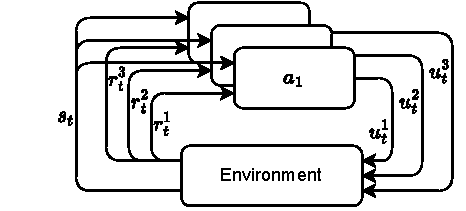
\includegraphics[width=.8\textwidth]{tex_thesis/figures/ch2/SG.pdf}
    \caption{Interaction of three agents with the environment in a stochastic game \citep{stochasticGames}. Agents $i \in \{1,..,n\}$ have access to the state $s_t$ to select actions $u_t^i$. As a consequence, they each receive a reward $r_t^i$ and the environment transitions in a new state $s_{t+1}$.}
    \label{fig:ch2_sg}
\end{figure}

Before discussing the challenges of learning in an SG, we hereafter provide some comments about its definition. 
Since the transition function is defined as stochastic, the reward function is always based on the following state obtained.
Still, we sometimes denote it  $R(s_t, \mathbf{u_t}, i)$ irrespective of this new state to enhance readability.
Moreover, the expected return is often denoted $E_{\mathbf{\pi}} \left[ G_0 \right]$ leaving the initial state distribution $p$ and the transition function $P$ dependencies implicit.
An essential characteristic of MARL is that agents do not always observe the state $s_t$ of the environment entirely to select an action.
This partial observability is further developed in Section~\ref{sec:ch2_partial_observability}.
Finally, in the literature, an SG is sometimes called a Markov game (e.g. \citep{MarkovGames}).

When multiple agents learn in the environment, many challenges arise, and we describe four.
One challenge is the non-stationarity of the learning agents.
Since all agents learn, they all update their strategy over time.
One typical risk is that agents may adapt to the strategy of others in an infinite cycle, as in the rock-paper-scissor example of Chapter \ref{ch:introduction}.
One example solution to this problem is to find a Nash equilibrium \citep{nash1950equilibrium}.
Such equilibrium is obtained when no agents are interested in changing their policy, meaning that if one changes its policy, its sum of discounted rewards will decrease.
There is at least one Nash equilibrium.
When there are several, one may provide a better sum of discounted rewards to all agents than another.
Identifying the optimality of policies, which is connected to finding the best equilibria, is a significant challenge in MARL.
This task is often split into two challenges: finding and evaluating equilibria.
Both aspects remain pretty difficult.
To reach such an equilibrium, agents' objectives may change from finding the maximum sum of discounted rewards to obtaining the equilibrium.
This manuscript details these alternative solutions and their optimality in Part \ref{part:compet}.
Another challenge is called credit assignment.
As highlighted in the SG definition, despite providing individual rewards, they provide feedback characterising all agent's actions.
It is often challenging for an agent to credit its actions or the ones of others.
Finally, the number of agents is critical in a MARL problem and represents the fourth challenge.
Indeed, the size of the joint action space $|\mathcal{U}|$ scales exponentially with the number of agents.
As highlighted in this manuscript, many components of the MARL problem are built as a function of the joint action space.
A typical example is to decide if a joint policy is an equilibrium.
These four challenges represent the main challenges in MARL identified \cite{marl-book}.
As mentioned in the introduction, specific settings exist in MARL, and addressing these challenges can be eased when considering additional hypotheses on the structure of the stochastic game, as detailed in the next section.

\section{Multi-agent settings} 
\label{sec:ch2_multi_agent_settings}
The stochastic game definition proposed in Section~\ref{sec:ch2_stochastic_Game} provides a general framework for multi-agent systems.
A particular case is the stateless SG played by selecting a single action called the normal-form game.
These games are also called matrix games because a payoff matrix, a matrix of reward, can represent them.
This section defines the three specific settings commonly distinguished in MARL, and normal-form game examples will be provided to help provide intuition.
A typical example is the prisoner dilemma, and its payoff matrix is provided in Table \ref{table:ch2_prisonmatrix}.
When agent 0 chooses the action $B$, it receives a reward equal to 0 when agent 1 chooses the action $A$, provided in the bottom left corner.

\begin{table}
\centering
\begin{tabular}{cc|c|c|}
  & \multicolumn{1}{c}{} & \multicolumn{2}{c}{Agent 1}\\
  & \multicolumn{1}{c}{} & \multicolumn{1}{c}{$A$}  & \multicolumn{1}{c}{$B$} \\\cline{3-4}
   \multirow{2}*{\rotatebox[origin=r]{0}{Agent 0}}  & $A$ & $(-1, -1)$ & $(-5, 0)$ \\\cline{3-4}
                            & $B$ & $(0, -5)$ & $(-2, -2)$ \\\cline{3-4}
\end{tabular}
\caption{Prisoner dilemma payoff matrix.}
\label{table:ch2_prisonmatrix}
\end{table}

While MARL takes foundation in RL, it also takes foundation in game theory (GT) \citep{von1947theory} that provided this classification.
The difference in these settings is the relation between the rewards of agents \citep{marl-book}.
The first setting, cooperation, involves agents acting to achieve a common goal.
In this setting, agents typically share the same reward.
The second setting, competition, is the opposite, where agents pursue an opposing goal.
In this case, agents typically receive rewards that sum to a constant since the gain of one is equal to the retrofit of others.
The third setting is named general-sum and encompasses everything else.
The stochastic game provides a typical framework for a general-sum problem, while its definition is adapted when it is cooperative or competitive.
Not much detail will be provided here because these settings are the concern of further chapters.
Following this section, we develop more in-depth details about the single-agent setting in the next Section~\ref{sec:ch2_single_agent_RL}.

\subsection{Cooperation} 
\label{sec:ch2_Cooperation}
When agents share the same goal, they cooperate, and it is possible to model with a reward function providing a single reward for all agents instead of a different one per agent.
This is called "common reward games" in \citep{marl-book}.
Many problems can be considered as being a cooperative multi-agent setting.
Examples include robot coordination (e.g. in \citep{papoudakis2021benchmarking}), train scheduling (e.g., in \citep{mohanty2020flatland}), traffic control (e.g. in \citep{zhang2019cityflow}) but also games (e.g., Hanabi \citep{Bard_2020}).
\citet{oroojlooy2022review} provide a review of cooperative MARL, including a more detailed list of applications.
An example of a normal-form cooperative game with a payoff matrix is provided in Table \ref{table:ch2_coopmatrix}.

\begin{table}
\centering

\begin{tabular}{cc|c|c|}
  & \multicolumn{1}{c}{} & \multicolumn{2}{c}{Agent 1}\\
  & \multicolumn{1}{c}{} & \multicolumn{1}{c}{$A$}  & \multicolumn{1}{c}{$B$} \\\cline{3-4}
  \multirow{2}*{\rotatebox[origin=c]{0}{Agent 0}} & $A$ & $(-1, -1)$ & $(1, 1)$ \\\cline{3-4}
                            & $B$ & $(1, 1)$ & $(3, 3)$ \\\cline{3-4}
\end{tabular}
\caption{Payoff matrix of a cooperative normal-form game.}
\label{table:ch2_coopmatrix}
\end{table}


Part~\ref{part:coop} of this manuscript is dedicated to cooperative settings with a common reward.
In Chapter~\ref{ch:cooperation}, we provide the adaptation of the stochastic game definition to a cooperative setting, followed by examples of environments and methods to solve them.
In Chapter~\ref{ch:qvmix}, we present a method to solve such a setting, while in Chapter~\ref{ch:impmarl}, we present a suite of environments which frame a real-world application as a cooperative MARL problem.

\subsection{Competition} 
\label{sec:ch2_Competition}
When agents have opposite goals, they compete.
In competition, any action that benefits one agent incurs a retrofit to other ones.
This setting is also called a zero-sum game \citep{marl-book} because it is often modelled such that the rewards of all agents sum to a constant at any time.
In a two-agent zero-sum game, commonly known as a two-player zero-sum game in the game theory literature \citep{russel2010}, a classical implementation of the stochastic game is to have the reward function providing the same reward to all agents.
One agent aims to maximise it while the other tries to minimise it.
We also refer to this setting as fully competitive.
An example of a normal-form cooperative game with a payoff matrix is provided in Table \ref{table:ch2_competmatrix}.
A concrete example is chess with a single reward at the end of the game: $1$ if player 1 won, $0$ if player 1 lost or $1/2$ if players drew.
Player 2's goal would be to minimise this reward, while Player 1 wants to maximise it.
Other examples include card games (e.g. Poker \citep{poker}), board games (e.g. chess, shogi, and Go \citep{silver2018general} or Stratego \citep{stratego}) and video games (e.g. StarCraft II \citep{vinyals2019grandmaster}).
Part~\ref{part:compet} of this manuscript is not only dedicated to competitive settings but provides, in Chapter \ref{ch:competition}, many details on training agents in a competitive setting.

\begin{table}
\centering

\begin{tabular}{cc|c|c|}
  & \multicolumn{1}{c}{} & \multicolumn{2}{c}{Agent 1}\\
  & \multicolumn{1}{c}{} & \multicolumn{1}{c}{$A$}  & \multicolumn{1}{c}{$B$} \\\cline{3-4}
  \multirow{2}*{\rotatebox[origin=c]{0}{Agent 0}} & $A$ & $(0, 0)$ & $(-2, 2)$ \\\cline{3-4}
                            & $B$ & $(1, -1)$ & $(2, -2)$ \\\cline{3-4}
\end{tabular}
\caption{Payoff matrix of a competitive normal-form game.}
\label{table:ch2_competmatrix}
\end{table}

\subsection{General-sum} 
\label{sec:ch2_general_sum}
The third setting includes everything that is not fully cooperative or fully competitive.
Apriori, it is impossible to adapt the reward function of the general definition as no hypothesis can be made on the corresponding goals of agents.
The prisoner dilemma, whose payoff matrix is presented in Table \ref{table:ch2_prisonmatrix}, is an example of a not cooperative nor competitive normal-form game.
One of the best examples of the general-sum setting is autonomous driving \citep{dinneweth2022multi}, simulated, for example, in Nocturne \citep{nocturne2022}.

In this manuscript, we are interested in the mixed cooperative-competitive setting where two teams compete against each other.
Examples of this particular setting include games where two teams face each other (e.g., Dota 2 \citep{openai2019dota}).
We model such a setting with a reward function providing only two rewards, one per team.
Part~\ref{part:compet} is dedicated to this setting, and we study how methods designed for competition can work alongside cooperation ones.
We provide background in Chapter~\ref{ch:competition}, including necessary background from the competitive literature, and then detail our contribution in Chapter~\ref{ch:2teams}.

\section{Single-agent reinforcement learning} 
\label{sec:ch2_single_agent_RL}
When a single agent learns in the environment, it is called single-agent reinforcement learning (SARL).
The most significant part of the history of RL lies in this setting.
Indeed, the foundation of MARL relies on many works proposed initially in the single-agent framework.
In this section, we introduce the Markov decision process and discuss some fundamentals of RL, including model-based versus model-free, dynamic programming, value-based and policy-based methods.

\subsection{Markov decision process}
\label{sec:ch2_mdp}

The definition of a Markov decision process (MDP) can be obtained by considering a single agent in a stochastic game (see Section~\ref{sec:ch2_stochastic_Game}).
We, therefore, do not redefine the SG by removing the agent consideration but still present how this single agent interacts in an MDP in Figure~\ref{fig:ch2_mdp}.
Despite being alone, the agent's goal is the same as in an SG, to maximise the expected discounted return over a finite episode $\mathbb{E}_{\pi}\left[ G_0 \right]$.
To maximise its discounted return, the agent needs to learn an optimal policy $\pi^* = \argmax_\pi \mathbb{E}_{\pi}\left[ G_0 \right]$.
To evaluate a policy, we define the state value function $V^\pi(s) = \mathbb{E}_{\pi}\left[G_t|s_t=s\right]$ and the state-action value function $Q^\pi(s, u) = \mathbb{E}_{\pi}\left[G_t|s_t=s, u_t=u\right]$.
While it may appear meaningless for a single-agent environment, it is interesting to observe that the optimal policy is a Nash equilibrium.
Indeed, the agent can not profit from changing its policy.

An important property in MDP and SG that is not mentioned in the SG definition is that the next state depends only on the current state and action.
This is called the Markovian property.
It is important because it implies that a policy based solely on the current state is as good as one based on the history of states and actions.
Moreover, we defined the policy as the probability of taking action in a given state.
A particular case is a deterministic policy, denoted $\pi(s):\mathcal{S}\rightarrow\mathcal{U}$, or standardly $\mu(s)$.

\begin{figure}
    \centering
    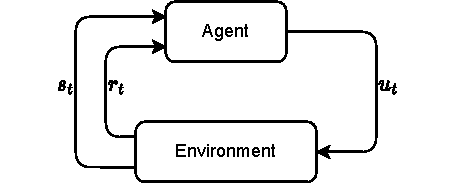
\includegraphics[width=.8\linewidth]{tex_thesis/figures/ch2/MDP.pdf}
    \caption{Interaction of agent with the environment in a Markov decision process \citep{sutton2018reinforcement}. The agent selects one action $u_t$ based on the state $s_t$. As a consequence, it receives a reward $r_t$ and the environment transitions in a new state $s_{t+1}$.}
    \label{fig:ch2_mdp}
\end{figure}

Usually, two families of methods are identified in RL to learn this optimal policy.
Value-based methods learn a value function and derive the policy from it, while policy-based methods directly learn a policy.
But before diving into these details, we first discuss whether the model is known, leading to model-based RL, sometimes categorised as a third family of RL methods.

\subsection{Model-based or model-free}
\label{sec:ch2_model_based_vs_model_free}

When solving an MDP, we distinguish methods based on the knowledge of action outcomes.
Indeed, knowing the model of the MDP, one can simulate the environment to evaluate policies \citep{sutton2018reinforcement}.
``A model is a form of reversible access to the MDP dynamics (known or learned)'' \citep{moerland2023model}.
This reversible access means that the agent can execute an action in any state of the MDP and access the outcome anytime.
Learning by trial and error without a model is referred to as model-free RL, and this manuscript focuses on methods following this approach.

Planning and RL are two different approaches to finding an MDP's solution when the model is known.
They differ in how they represent the solution.
Planning is the historical one, where methods build a local representation of their solution, typically by evaluating policies or resolving an optimisation problem around a given state and discarding them after taking action.
It typically does not involve learning anything.
This is how DeepBlue \citep{campbell2002deep} defeated human champions without learning by evaluating the outcome of many actions before taking each action.
Conversely, the RL approach stores a global solution, typically a learned policy or a state-action value function, whether it can access the model.
This leads to the distinction between model-based RL and planning of \cite{moerland2023model}.
Both have access to the model, but the former learns a global solution while the latter computes local ones.
Knowing the model or learning it is not considered in these definitions of planning and RL, and both exist: learning the model and the solution or learning the model and planning a solution based on it.

This distinction between planning and RL does not always agree because, in some methods, a global value function is learned to compute a local representation of the solution, such as in AlphaZero \citep{silver2018general}, considered as model-based RL by some and planning by others.
We finally refer to the work of \cite{moerland2023model} that provides many keys to bridge the gap between RL and planning, between model-based and model-free.
Nevertheless, the following section introduces dynamic programming, methods requiring a model to compute the optimal policy and providing foundations for the model-free methods.

\subsection{Dynamic programming}
Dynamic programming (DP) \citep{bellman1966dynamic} methods compute the optimal policies given a model of an MDP \citep{sutton2018reinforcement}.
First, we present the Bellman equation to provide some intuitions to help understand later methods and discuss dynamic programming methods.
They are obtained by developing value functions, highlighting their recursive relationships, for any policy $\pi$ and $\forall s, u$,
\begin{equation}
\label{eq:ch2_V_2}
\begin{split}
    V^\pi(s)= \mathbb{E}_{\pi}\left[G_t|s_t=s\right] & = \mathbb{E}_{\pi}\left[r_t + \gamma V^\pi(s_{t+1})|s_t=s\right],
\end{split}
\end{equation}
and,
\begin{equation}
\label{eq:ch2_Q_2}
\begin{split}
    Q^\pi(s, u) = \mathbb{E}_{\pi}\left[G_t|s_t=s, u_t=u\right] & = \mathbb{E}_{\pi}\left[r_t + \gamma V^\pi(s_{t+1})|s_t=s, u_t=u \right].
\end{split}
\end{equation}

From these equations, a policy $\pi'$ is better than another $\pi$ if $V^{\pi'}(s)>V^\pi(s)$.
The policy that is better than all others is the optimal policy.
While there can be several optimal policies, all are denoted by $\pi^*$, and their state value function $V^{\pi^*}(s)$ is the same $\forall s$.
The optimal policies are the unique solution of the Bellman optimality equations, $\forall s, u$,
\begin{equation}
\label{eq:ch2_bellmanV}
    V^{\pi^*}(s) = \max_{\pi}V^\pi(s) = \max_u \mathbb{E}_{\pi^*}[r_t + \gamma V^{\pi^*}(s_{t+1})| s_t=s, u_t=u],
\end{equation}
and,
\begin{equation}
\label{eq:ch2_bellmanQ}
    Q^{\pi^*}(s, u) =  \max_{\pi}Q^\pi(s, u) = \mathbb{E}_{\pi^*}[r_t + \gamma \max_{u'} Q^{\pi^*}(s_{t+1}, u') |s_t=s, u_t=u].
\end{equation}
The optimality equations given in Equation \ref{eq:ch2_bellmanV} represent a system of $|\mathcal{S}|$ equations with $|\mathcal{S}|$ unknown, and solving this system would allow one to compute the optimal policy.
This can also be done with the system defined in Equation \ref{eq:ch2_bellmanQ}.
The condition is, of course, to have reversible access to the MDP model.
Solving either system is usually not considered for computational reasons.
Therefore, this manuscript presents methods for computing an approximate solution to the Belman optimality equations.

DP is an approach that computes the solutions by iteratively updating approximations until they converge.
DP can solve Equation \ref{eq:ch2_V_2} by updating estimates $v_k$ with $v_{k+1}(s) = \sum_{u} \pi(u|s) \sum_{s'} P(s', s, u) (R(s', s, u) + \gamma v_k(s'))$, where $v_0(s)$ can have arbitrary values except for terminal states that are required to equal 0.
This is called iterative policy evaluation and is proven to converge if $k\rightarrow\infty$.
Policy evaluation allows the refinement of any given policy $\pi$ by exploiting Equation \ref{eq:ch2_Q_2} to evaluate other actions than $\pi(s)$ using $Q^\pi(s, u) =  \sum_{s'} P(s', s, u) (R(s', s, u) + \gamma v_k(s'))$. 
This is called policy improvement.
Alternating policy evaluation and improvement allows the iterative computation of the optimal policy, called policy iteration.
Policy iteration convergence time can be a significant drawback in policy iteration.
However, the convergence guarantee can be kept while combining evaluation and improvement, leading to an approximation called value iteration $v_{k+1}(s) = \max_u \sum_{s'} P(s', s, u) (R(s', s, u) + \gamma v_k(s'))$.
\cite{sutton2018reinforcement} provides many more details about these DP methods.

In addition to requiring the model knowledge $P$ and $R$, the complexity of computing all these values increases with the size of the state and the action spaces, often referred to as the curse of dimensionality, which may limit their usage.
\cite{sutton2018reinforcement} claim that this take is somehow mistaken, explaining that DP has a polynomial complexity with $|\mathcal{S}|$ and $|\mathcal{U}|$ and could scale to large spaces.
Nevertheless, computing them is impossible for continuous spaces without discretising the spaces.

We are interested in model-free methods because accessing the model knowledge can be challenging.
One possibility is to estimate the state value function of a given policy with Monte-Carlo estimations.
Such evaluation of a state relies on playing many episodes by plating actions provided by the policy to determine its average return.
This method also converges according to the law of large numbers.
Since the model is unknown, improving policies like in DP is impossible, but Monte-Carlo simulations can be adapted to estimate state-action value functions.
Again, \citep{sutton2018reinforcement} provides many more details.
One important drawback in Monte-Carlo methods is that the estimation requires waiting for the completion of episodes to update estimations.
An alternative approach, model-free and using episode samples, is called temporal difference (TD) learning.
It immedialy updates the estimation using $v_{k+1}(s_t) = v_k(s_t) + \alpha [R(s_{t+1}, s_t, u_t) + \gamma v_k(s_{t+1}) - v_k(s_t)]$ where $\alpha$ controls the update size.
TD-Learning is the foundation of the value-based methods introduced in the following section.

\subsection{Value-based methods} \label{sec:ch2_value_based_methods}
Value-based methods are designed to learn value functions.
Maybe one of the most common methods in model-free RL is Q-learning \citep{watkins1992q}, where the state-action value function learned is the optimal one defined as $Q^{\pi^*}(s, u)=\max_{\pi}Q^\pi(s, u)$.
This enables the agent to greedily select the action following the deterministic policy $\pi^*(s)=\argmax_u Q^{\pi^*}(s, u)$.

Q-learning is a tabular method because it maintains $Q(s, u)$ estimations in a table, one value for each state-action pair.
It updates these estimations based on themselves, called bootstrapping, and is based on temporal difference (TD) learning \citep{sutton2018reinforcement}.
Following the update 
\begin{equation}
\label{eq:ch2_QLearning}
    Q(s_t, u_t) \leftarrow Q(s_t, u_t) + \alpha \left[ r_t + \gamma \max_u Q(s_{t+1}, u) - Q(s_t, u_t) \right],
\end{equation}
it is possible to repeatedly update the estimation $Q(s, u)$ while observing new transitions by adding the temporal difference weighted by a learning rate $\alpha$ controlling the update size.

It is important to denote that this algorithm allows approximating $Q^{\pi^*}(s, u)$ independently of the policy used to sample transitions ($s_t, u_t, r_t, s_{t+1}$).
These transition samples are typically generated with an $\epsilon$-greedy policy that takes a random action instead of the greedy one with a probability $\epsilon$, whereas the greedy policy selects the action maximising $Q$.
This is a characteristic of the off-policy methods, as opposed to the on-policy method, which improves the current policy based on samples only from the current policy.
This manuscript considers only value-based methods that are off-policy, but on-policy methods are discussed further in Section~\ref{sec:ch2_policy_based_methods}.
To cite one, SARSA is a well-known on-policy value-based method \citep{sutton2018reinforcement}.

Despite being off-policy, this iterative process highlights the exploration-exploitation dilemma in RL.
Either the agent only plays the action that maximises its currently learned value function, which it exploits, or it chooses a different action and explores the possible outcomes.
Balancing between exploration and exploitation is a crucial parameter to train agents.

Back to Q-learning, the table size increases as the state-action space size increases.
Therefore, it can become impractical to compute an estimate of $Q(s, u)$ for each state-action pair, requiring function approximations.
Aside from the generalisation problem, storing a table for continuous spaces is also impossible.
Various function approximators exist, but we restrict ourselves to neural networks in this manuscript.

A neural network is a function $f_\theta: \mathcal{X} \rightarrow \mathcal{Y}$ that maps an input ($\in\mathcal{X}$) to an output ($\in\mathcal{Y}$) based on its parameters $\theta$: $y = f(x;\theta)$.
These parameters define a composition of differentiable functions, linear or not, allowing optimising the parameters by following the gradient of an objective, commonly called a loss function $\mathcal{L}(\theta)$.
To minimise the loss, parameters can be updated by gradient descent: $\theta_{k+1} = \theta_k - \alpha \nabla \mathcal{L}(\theta_k)$.
Optimising a neural network is also referred to as training it.
Many loss functions exist to train neural networks, depending on the function to be approximated.
Nowadays, neural networks are very large, leading to the name of deep learning.
We refer to \citep{zhang2023dive} or \citep{prince2023understanding} for many more details.
Finally, RL with neural networks is called deep reinforcement learning, e.g. in \citep{introDeepRL}.
As it became common to use neural networks in RL, we decided to remove the word "deep" from the taxonomy, as the title of this manuscript should be "Contributions to deep multi-agent reinforcement learning".
In the following, we introduce how to train such networks to approximate a value function and, in Section~\ref{sec:ch2_policy_based_methods}, to approximate a policy.

A standard method in RL, referred to as deep Q-network (DQN) \citep{Mnih2015}, is to approximate $Q(s, u)$ with a neural network $\theta$.
This can be achieved by minimising the loss 
\begin{equation}
\label{eq:ch2_dqnloss}
    \mathcal{L}(\theta) = \mathbb{E}_B \big[\big(r_{t} + \gamma \max_u Q(s_{t+1}, u; \theta')- Q(s_{t}, u_{t}; \theta)\big)^{2}\big]
\end{equation}
where $B$ is the replay buffer and $\theta'$ is the target network.
The replay buffer $B$ stores transitions $\langle s_{t},u_{t},r_{t},s_{t+1}\rangle$ from which batches of transitions are sampled to update $\theta$ \citep{lin1992self}.
This replay buffer allows updating the neural network with past transitions.
The target network $\theta'$ is a copy of $\theta$ updated periodically that reduces the moving target problem as $\theta$ is updated several times before updating $\theta'$, e.g., in \citep{Mnih2015}.

In both Equations~\ref{eq:ch2_QLearning} and~\ref{eq:ch2_dqnloss}, the $\max$ operator can introduce some positive bias. 
To overcome this bias, a method called Double Q-learning \citep{hasselt2010double}, and adapted to Q-learning with approximations \citep{van2016deep}, consists in selecting the action that maximises the updated $Q(., \theta)$ to compute the target state-action value.
The corresponding loss is 
\begin{equation}
    \label{eq:ch2_doubleQ}
    \mathcal{L}(\theta) = \mathbb{E}_{B} \big[\big(r_{t} + \gamma Q(s_{t+1}, \argmax_u Q(s_{t+1}, u;\theta) ; \theta')- Q(s_{t}, u_{t}; \theta)\big)^{2}\big].
\end{equation}

Double Q-learning, also called DDQN, is one of the possible improvements of DQN, and we refer to the Rainbow paper \citep{hessel2018rainbow} that addresses several others.
To cite one, the extension to distributional RL, which approximates distributions instead of expected returns, can be of interest \citep{bellemare2017distributional, THEATE2023199}. 

\subsection{Policy-based methods} \label{sec:ch2_policy_based_methods}
Policy-based methods are designed to learn the policy.
In this manuscript, we restrict to the subclass of policy gradient methods where a neural network parametrised by $\theta$ approximates a differentiable policy $\pi_\theta=\pi(u|s;\theta)$.
Policy gradient methods hence update $\theta$ to find the optimal policy that maximises the expected return denoted as  $J(\pi_\theta) = \mathbb{E}_{\pi_\theta, p}[G_0]$.
Maybe one of the first methods is REINFORCE \citep{williams1992simple}, which updates $\theta = \theta + \alpha \nabla_\theta J(\pi_\theta)$ by estimating the gradient with Monte-Carlo given the policy gradient theorem \citep{sutton1999policy} 
\begin{equation}
\label{eq:ch2_reinforce_grad}
    \nabla_\theta J(\pi_\theta) = \nabla_\theta \mathbb{E}_{\pi_\theta}[G_0] = \mathbb{E}\left[\sum_{t=0}^{T-1} Q^{\pi_\theta}(s_t, u_t) \nabla_\theta \log \pi(u_t|s_t;\theta)\right].
\end{equation}

Estimating $Q(s_t, u_t)$ instead of computing it is a solution proposed by the actor-critic methods \citep{sutton1999policy,konda1999actor}.
This type of method expands upon REINFORCE by incorporating a second neural network, called the critic and denoted by $\phi$, that estimates $Q(s_t, u_t;\phi)$ while the actor is the parametrised policy $\pi(u|s;\theta)$.
The new gradient provided by incorporating the critic is
\begin{equation}
\label{eq:ch2_Q_actor_crit}
    \nabla_\theta J(\pi_\theta) = \mathbb{E}\left[\sum_{t=0}^{T-1} Q(s_t, u_t;\phi) \nabla_\theta \log \pi(u_t|s_t;\theta)\right].
\end{equation}

Moreover, a baseline can be injected into the gradient to reduce variance without changing the gradient's expectation.
Usually, the baseline is  $V(s)$, independent of the action taken, and $Q(s, u;\phi)$ is replaced by the advantage function $A(s,u; \phi)$ \citep{10.5555/2074022.2074088}, leading to

\begin{align}
\begin{split}
\label{eq:ch2_baseline_actor_crit}
    \nabla_\theta J(\pi_\theta)
    & = \mathbb{E}\left[\sum_{t=0}^{T-1} [Q(s_t, u_t) - V(s_t)] \nabla_\theta \log \pi(u_t|s_t;\theta)\right]\\
    & = \mathbb{E} \left[\sum_{t=0}^{T-1} A(s_t, u_t; \phi) \nabla_\theta \pi(s_t, u_t; \theta)\right].
\end{split}
\end{align}

To avoid approximating both $Q$ and $V$, it is possible to estimate the advantage with only one neural network either by $A(s_t,u_t; \phi)=Q(s_t, u_t;\phi)-\sum_u \pi(u|s_t;\theta) Q(s_t,u; \phi)$ or by $A(s_t,u_t; \phi)=r_t +\gamma V(s_{t+1};\phi) - V(s_t;\phi)$.
This critic is often trained with value-based methods, such as the ones defined in Section~\ref{sec:ch2_value_based_methods}.
This is why actor-critic methods are sometimes described as a mix between value-based and policy-based methods.

Nowadays, advanced policy-based methods relying on the actor-critic paradigm appear to be the most successful.
We can cite trust region policy optimisation (TRPO) \citep{schulman2015trust} and its variant proximal policy optimisation (PPO) \citep{schulman2017ppo}.
Both methods rely on a controlled policy update by constraining the loss of REINFORCE defined in Equation~\ref{eq:ch2_reinforce_grad}.

Finally, policy gradient and actor-critic algorithms also need some form of exploration, usually implemented by adding a penalisation term in the loss function. 
An example is entropy regularisation \citep{williams1991function}, where a low entropy of the policy outcomes is penalised.
In this context, \cite{bolland2024behind} demonstrates that such techniques change the learning objective and increase the probability of updating the policy toward the optimal one.

\section{Partial observability} \label{sec:ch2_partial_observability}

As defined in previous sections, the Markov decision process and the stochastic game are fully observable.
Agents have complete access to the state $s$ of the environment and perceive it without uncertainty.
In real-world applications, it is not always possible to consider this feasible.
Anyone can develop ideas of a partially observable environment, especially given our definition of agents ``acting upon information it perceives''.

Starting with SARL, the Markov decision process is said to be a partially observable MDP (POMDP) \citep{KAELBLING199899} when the agent can only access incomplete information about the state.
The definition of a POMDP is obtained easily from the MDP definition of Section~\ref{sec:ch2_mdp} by adding an observation space $\mathcal{Z}$ and an observation function $O:\mathcal{S} \rightarrow \Delta(\mathcal{Z})$, mapping a state and an observation to the probability of observing the latest.
The corresponding interaction diagram of a POMDP is presented in Figure \ref{fig:ch2_pomdp}.

\begin{figure}
    \centering
    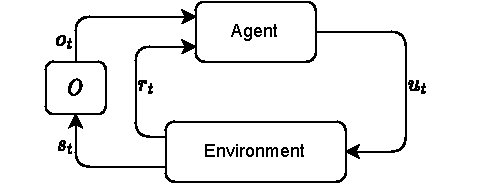
\includegraphics[width=.8\linewidth]{tex_thesis/figures/ch2/POMDP.pdf}
    \caption{Interaction of agent with the environment in a partially observable Markov decision process \citep{KAELBLING199899}. The agent does not have access to the state $s_t$ but to an observation $o_t$ defined by the observation function $O$. Based on $o_t$, it selects one action $u_t$. As a consequence, it receives a reward $r_t$ and the environment transitions in a new state $s_{t+1}$.}
    \label{fig:ch2_pomdp}
\end{figure}

As explained in Section \ref{sec:ch2_mdp}, policies are solely based on the current state in an MDP, thanks to the Markovian property.
In a POMDP, the agent's policy $\pi$ can no longer be a function of the state.
Moreover, the observation does not necessarily hold the Markovian property, and acting only based on the current observation could be suboptimal.
Therefore, the policy is commonly a function of the history of past observations and past actions $\tau_t=(\mathcal{Z} \times \mathcal{U})^t$, in addition to the current observation, and is denoted $\pi(u_t|\tau_t,o_t): (\mathcal{Z} \times \mathcal{U})^t \times \mathcal{Z} \rightarrow \Delta(\mathcal{U})$.
Some authors implicitly include the current observation in $\tau$, allowing them to write $\pi(u|\tau)$ and $Q(\tau,u)$.
We sometimes do it to improve readability as well.

To solve a POMDP, a solution is to compute the policy based on a belief $b(s)=\mathbb{P}(s|\tau,o)$, the probability of being in a given state, knowing the history of observations and actions.
As in the different methods previously defined, the belief can be implicitly approximated with recurrent neural networks (RNN), such as GRU \citep{Chung2014EmpiricalModeling} or LSTM \citep{Hochreiter1997LongMemory}.
These networks typically take time series as input and maintain a hidden state, updated at each time step of one time series, which can be considered a memory.
RNNs have many applications, and in POMDP, their hidden state allows to maintain a memory akin to a belief without processing the whole history at each time step.
Using RNNs to compute policies is thus a common practice in POMDP, resulting in recurrent policies.
It has demonstrated convincing results, such as in recurrent policy gradients \citep{wierstra2010recurrent} or in deep recurrent Q-network (DRQN) \citep{Hausknecht2015DeepMDPs}.
We suggest readers interested in details read the pedagogical paper of \cite{lambrechts2022recurrent}.
This paper demonstrates that the correlation between the hidden state of RNNs, used to approximate policies, and the belief increases as the training progresses.

Adding partial observability in the definition of the stochastic game leads to the most general framework of MARL, the partially observable stochastic game (POSG) \citep{hansen2004dynamic}.
Its definition is obtained by adding a set of $n$ observation spaces $\mathcal{Z}$ and a set of $n$ observation functions $\mathcal{O}$ in the definition of the SG.
A shortcut in this manuscript, and sometimes in the literature, is to consider that these two sets $\mathcal{Z}$ and $\mathcal{O}$ are singleton, such that the observation function $O:\mathcal{S} \times \mathcal{A} \rightarrow \Delta(\mathcal{Z})$ is the same for all agents.
An agent's belief in a POSG should be considered differently from that in a POMDP \citep{DecPomdp}.
This is because, with only the agent's history, it is impossible to compute a belief of the state that is sufficient to take optimal actions.
However, it would be possible to achieve this by having access to the histories of all agents.
Even when agents can fully observe the current state, they may not observe the actions previously taken by others.
However, this manuscript does not address multi-agent belief, and we refer to \citep{DecPomdp} for more details.
In a POSG, we consider that an agent's policy is a function $\pi^{a}(u_t^{a}|\tau_t^{a},o_t^{a}): (\mathcal{Z}^a \times \mathcal{U}^a)^t \times \mathcal{Z} \rightarrow \Delta(\mathcal{U}^a)$, which maps its history $\tau_t^{a} \in (\mathcal{Z}^a \times \mathcal{U}^a)^{t}$ and its current observation $o_t^{a}$ to the probability of taking action $u_t^{a}$.
As in SARL, such a policy is commonly a recurrent policy approximated with RNN.
